% Workshop build (NeurIPS 2026 style) for "Evaluation of Interactive Agents"
% @ NeurIPS 2026 (submission deadline Aug 29, 2026 AoE; CFP asks for the
% official NeurIPS 2026 LaTeX style, up to 9 pages for full papers excluding
% references and appendices; non-archival).
%
% Compiled by default in SUBMISSION mode (anonymized authors + line numbers),
% which is what gets uploaded to OpenReview if the finalized CFP confirms
% double-blind review. If the workshop turns out to be single-blind, switch
% the package options to [final] before submitting.
\documentclass{article}

\usepackage[nonatbib]{neurips_2026}

\usepackage[utf8]{inputenc}
\usepackage[T1]{fontenc}
\usepackage{graphicx}
\usepackage{amsmath}
\usepackage{amssymb}
\usepackage{booktabs}
\usepackage{multirow}
\usepackage[breaklinks=true,bookmarks=false]{hyperref}

\graphicspath{{figures/}}

% Workshop build: relocate three exploratory figures to the appendix
% (IAEval counts pages excluding references and appendices).
\newif\ifworkshopbuild
\workshopbuildtrue

% Every results number comes from committed artifacts via generated tables;
% see scripts/p10_render_paper_tables.py. Do not hand-type result numbers.
% AUTO-GENERATED by scripts/p10_render_paper_tables.py — do not edit
\newcommand{\LeakGoalMain}{24\%}
\newcommand{\LeakGoalMax}{85\%}
\newcommand{\LeakEpMain}{2\%}
\newcommand{\ExpBvsA}{$+0.051$ [+0.020, +0.081]}
\newcommand{\ExpBvsAp}{0.0043}
\newcommand{\ExpBvsAHolm}{0.017}
\newcommand{\ExpDhvsA}{$+0.045$ [+0.011, +0.085]}
\newcommand{\ExpDhvsAp}{0.0227}
\newcommand{\ExpDhvsAHolm}{0.068}
\newcommand{\ExpDtvsB}{$-0.036$ [-0.077, +0.005]}
\newcommand{\ExpDtvsBp}{0.114}
\newcommand{\ExpBvsApooled}{0.0002}
\newcommand{\TypeIPooled}{21.2\%}
\newcommand{\TypeIClustered}{5.1\%}
\newcommand{\TypeISims}{1000}
\newcommand{\TypeIProc}{55\%}
\newcommand{\ExpEtoEPredvsA}{$+0.016$ [-0.017, +0.052]}
\newcommand{\ExpEtoEPredvsAp}{0.424}
\newcommand{\ExpEtoEOraclevsA}{$+0.037$ [+0.005, +0.076]}
\newcommand{\ExpEtoEGap}{$-0.021$ [-0.041, -0.003]}

\providecommand{\ConfBvsA}{\textbf{[PENDING]}}
\providecommand{\ConfBvsAp}{\textbf{[PENDING]}}
\providecommand{\ConfBvsAHolm}{\textbf{[PENDING]}}
\providecommand{\ConfDhvsA}{\textbf{[PENDING]}}
\providecommand{\ConfDhvsAp}{\textbf{[PENDING]}}
\providecommand{\ConfDhvsAHolm}{\textbf{[PENDING]}}
\providecommand{\ConfDtvsB}{\textbf{[PENDING]}}
\providecommand{\ConfDtvsBp}{\textbf{[PENDING]}}
\providecommand{\ConfDtvsBHolm}{\textbf{[PENDING]}}
\providecommand{\ConfEtoEvsA}{\textbf{[PENDING]}}
\providecommand{\ConfEtoEvsAp}{\textbf{[PENDING]}}
\providecommand{\ConfEtoEvsAHolm}{\textbf{[PENDING]}}
\providecommand{\ConfAhit}{\textbf{[PENDING]}}
\providecommand{\ConfBhit}{\textbf{[PENDING]}}
\providecommand{\ConfAparse}{\textbf{[PENDING]}}
\providecommand{\ConfEtoEOracle}{\textbf{[PENDING]}}
\providecommand{\ConfEtoEPred}{\textbf{[PENDING]}}
\providecommand{\ConfEtoEGap}{\textbf{[PENDING]}}
\providecommand{\ConfStageOneAcc}{\textbf{[PENDING]}}
\providecommand{\ConfBvsALtwo}{\textbf{[PENDING]}}
\providecommand{\ConfBvsALtwop}{\textbf{[PENDING]}}

\title{When Does Action-Type Supervision Help GUI Grounding?\\
Separating Real Effects from Evaluation Artifacts}

\author{%
  Aadi Chauhan\\
  Stanford University\\
  \texttt{aadic@stanford.edu}
  \And
  Arthur Ilyasov\\
  Stanford University\\
  \texttt{ailyasov@stanford.edu}
}

\begin{document}

\maketitle

%%%%%%%%% ABSTRACT
\begin{abstract}
GUI agents must predict an action type (\emph{click}, \emph{scroll},
\emph{type}, \ldots) and a spatial target from a screenshot and an
instruction. We study whether explicitly factoring these decisions helps a
2B-parameter agent, via a matched-compute comparison of five conditioning
mechanisms on Qwen2-VL: a flat baseline (A), an auxiliary action-type loss
(B), hard routing (C), an additive embedding hook (D-hook), and the
prepended learned action embedding our original proposal advocated
(D-token). Equally central, we report how our own first evaluation of this
question misled us in three distinct ways, each of which we diagnose,
quantify, and repair: (i) injecting conditioning via
\texttt{inputs\_embeds} silently bypasses Qwen2-VL's M-RoPE position path
and manufactured an $8\sigma$ \emph{false negative}; (ii) train/validation
splits taken as consecutive slices of one episode stream leaked shared task
goals (\LeakGoalMain{} of validation steps at the headline setting, up to
\LeakGoalMax{} at scale); and (iii) a paired bootstrap that pooled
(seed, example) predictions as independent units was anti-conservative,
rejecting a true clustered null \TypeIPooled{} of the time at nominal
5\% (an episode-clustered replacement achieves \TypeIClustered{}). After the
statistical repair, the auxiliary-loss effect survives on the historical
data (B$-$A hit@0.10 \ExpBvsA{}, permutation $p=\ExpBvsAp$, versus the
invalid pooled $p=\ExpBvsApooled$); we then retrain all variants on frozen
goal-disjoint splits and evaluate once on an untouched test set under a
prespecified analysis. On that test set, B$-$A is \ConfBvsA{} (Holm
$p=\ConfBvsAHolm$) and the end-to-end predicted-type pipeline versus A is
\ConfEtoEvsA{} (Holm $p=\ConfEtoEvsAHolm$). The mechanism our proposal bet
on is refuted as the winner: D-token is causally used at inference (wrong
or zeroed embeddings severely hurt) yet never beats the plain auxiliary
loss, and exploratory per-class decompositions locate the gain in
click-vs-scroll/type disambiguation rather than field localization. We release the frozen
splits, per-example predictions, and the clustered-inference code; we argue
that offline step-level grounding studies at this scale are unusually easy
to contaminate, and that the three artifacts we document are likely present
in other evaluations.
\end{abstract}

%%%%%%%%% BODY TEXT
\section{Introduction}

A GUI agent maps a screenshot and a natural-language instruction to a
low-level action: a type (\emph{click}, \emph{scroll}, \emph{type},
\emph{drag}, \ldots) and, for spatial actions, a pixel-level target.
State-of-the-art native agents (UI-TARS~\cite{uitars},
OS-Atlas~\cite{osatlas}, SeeClick~\cite{seeclick}, ShowUI~\cite{showui})
emit both in one autoregressive stream, entangling the two decisions. A
documented failure mode follows: commit to the wrong action type, then
ground \emph{coherently} within the wrong semantic frame -- scrolling past a
visible target instead of clicking it. This motivated our original
hypothesis, formulated as an architecture bet: a learned action-type
embedding, prepended to the instruction, should let a grounding model
condition on \emph{what} before deciding \emph{where}, and should help most
in low data.

This paper reports what happened when we tested that bet carefully, and it
has two intertwined subjects. The first is the scientific question:
\emph{when does action-type supervision change GUI grounding, and through
which mechanism?} The second is methodological: \emph{which implementation
and evaluation choices can create a false appearance of benefit or harm in
studies of exactly this kind?} We came to the second subject involuntarily
-- three separate artifacts in our own pipeline each produced a wrong
conclusion at some point during the project -- and we believe the
post-mortem is at least as useful to practitioners as the object-level
result.

Concretely, we compare five matched-compute Stage-2 conditioning mechanisms
on Qwen2-VL-2B~\cite{qwen2vl} with LoRA, over AITW~\cite{aitw} with a
Mind2Web~\cite{mind2web} cross-dataset control, preceded by a Stage-1
action-type classifier study. Our contributions:

\begin{itemize}
\item \textbf{A controlled answer to the factorization question.}
Auxiliary action-type supervision (B) improves grounding where action type
is spatially predictive; the effect vanishes on a matched control where it
is not. The proposal's specific mechanism -- a routable prepended embedding
(D-token) -- is causally used by the trained model yet never outperforms
the far simpler auxiliary loss, refuting the architecture bet while
supporting the broader thesis.
\item \textbf{Three quantified evaluation pitfalls.} (1) A silent M-RoPE /
\texttt{inputs\_embeds} interaction that fabricated an $8\sigma$ false
negative; (2) episode-stream train/validation leakage that is invisible at
the episode level (\LeakEpMain{} of validation steps) but large at the
shared-task-goal level (\LeakGoalMain--\LeakGoalMax); (3) pseudo-replicated
significance testing whose anti-conservativeness we measure on synthetic
clustered nulls (\TypeIPooled{} type-I error at nominal 5\%).
\item \textbf{A repaired, releasable protocol.} Pinned-revision,
goal-disjoint frozen train/validation/test manifests with an untouched test
region beyond every historical data access; episode-clustered paired
inference with per-seed effects and validated calibration; and a
prespecified confirmatory analysis committed before test access. All
artifacts, per-example predictions, and analysis code are released.
\item \textbf{An honest confirmatory result.} We report the prespecified
untouched-test outcome for every primary contrast whatever its direction,
alongside the exploratory history that motivated it.
\end{itemize}

\begin{figure}[t]
\begin{center}
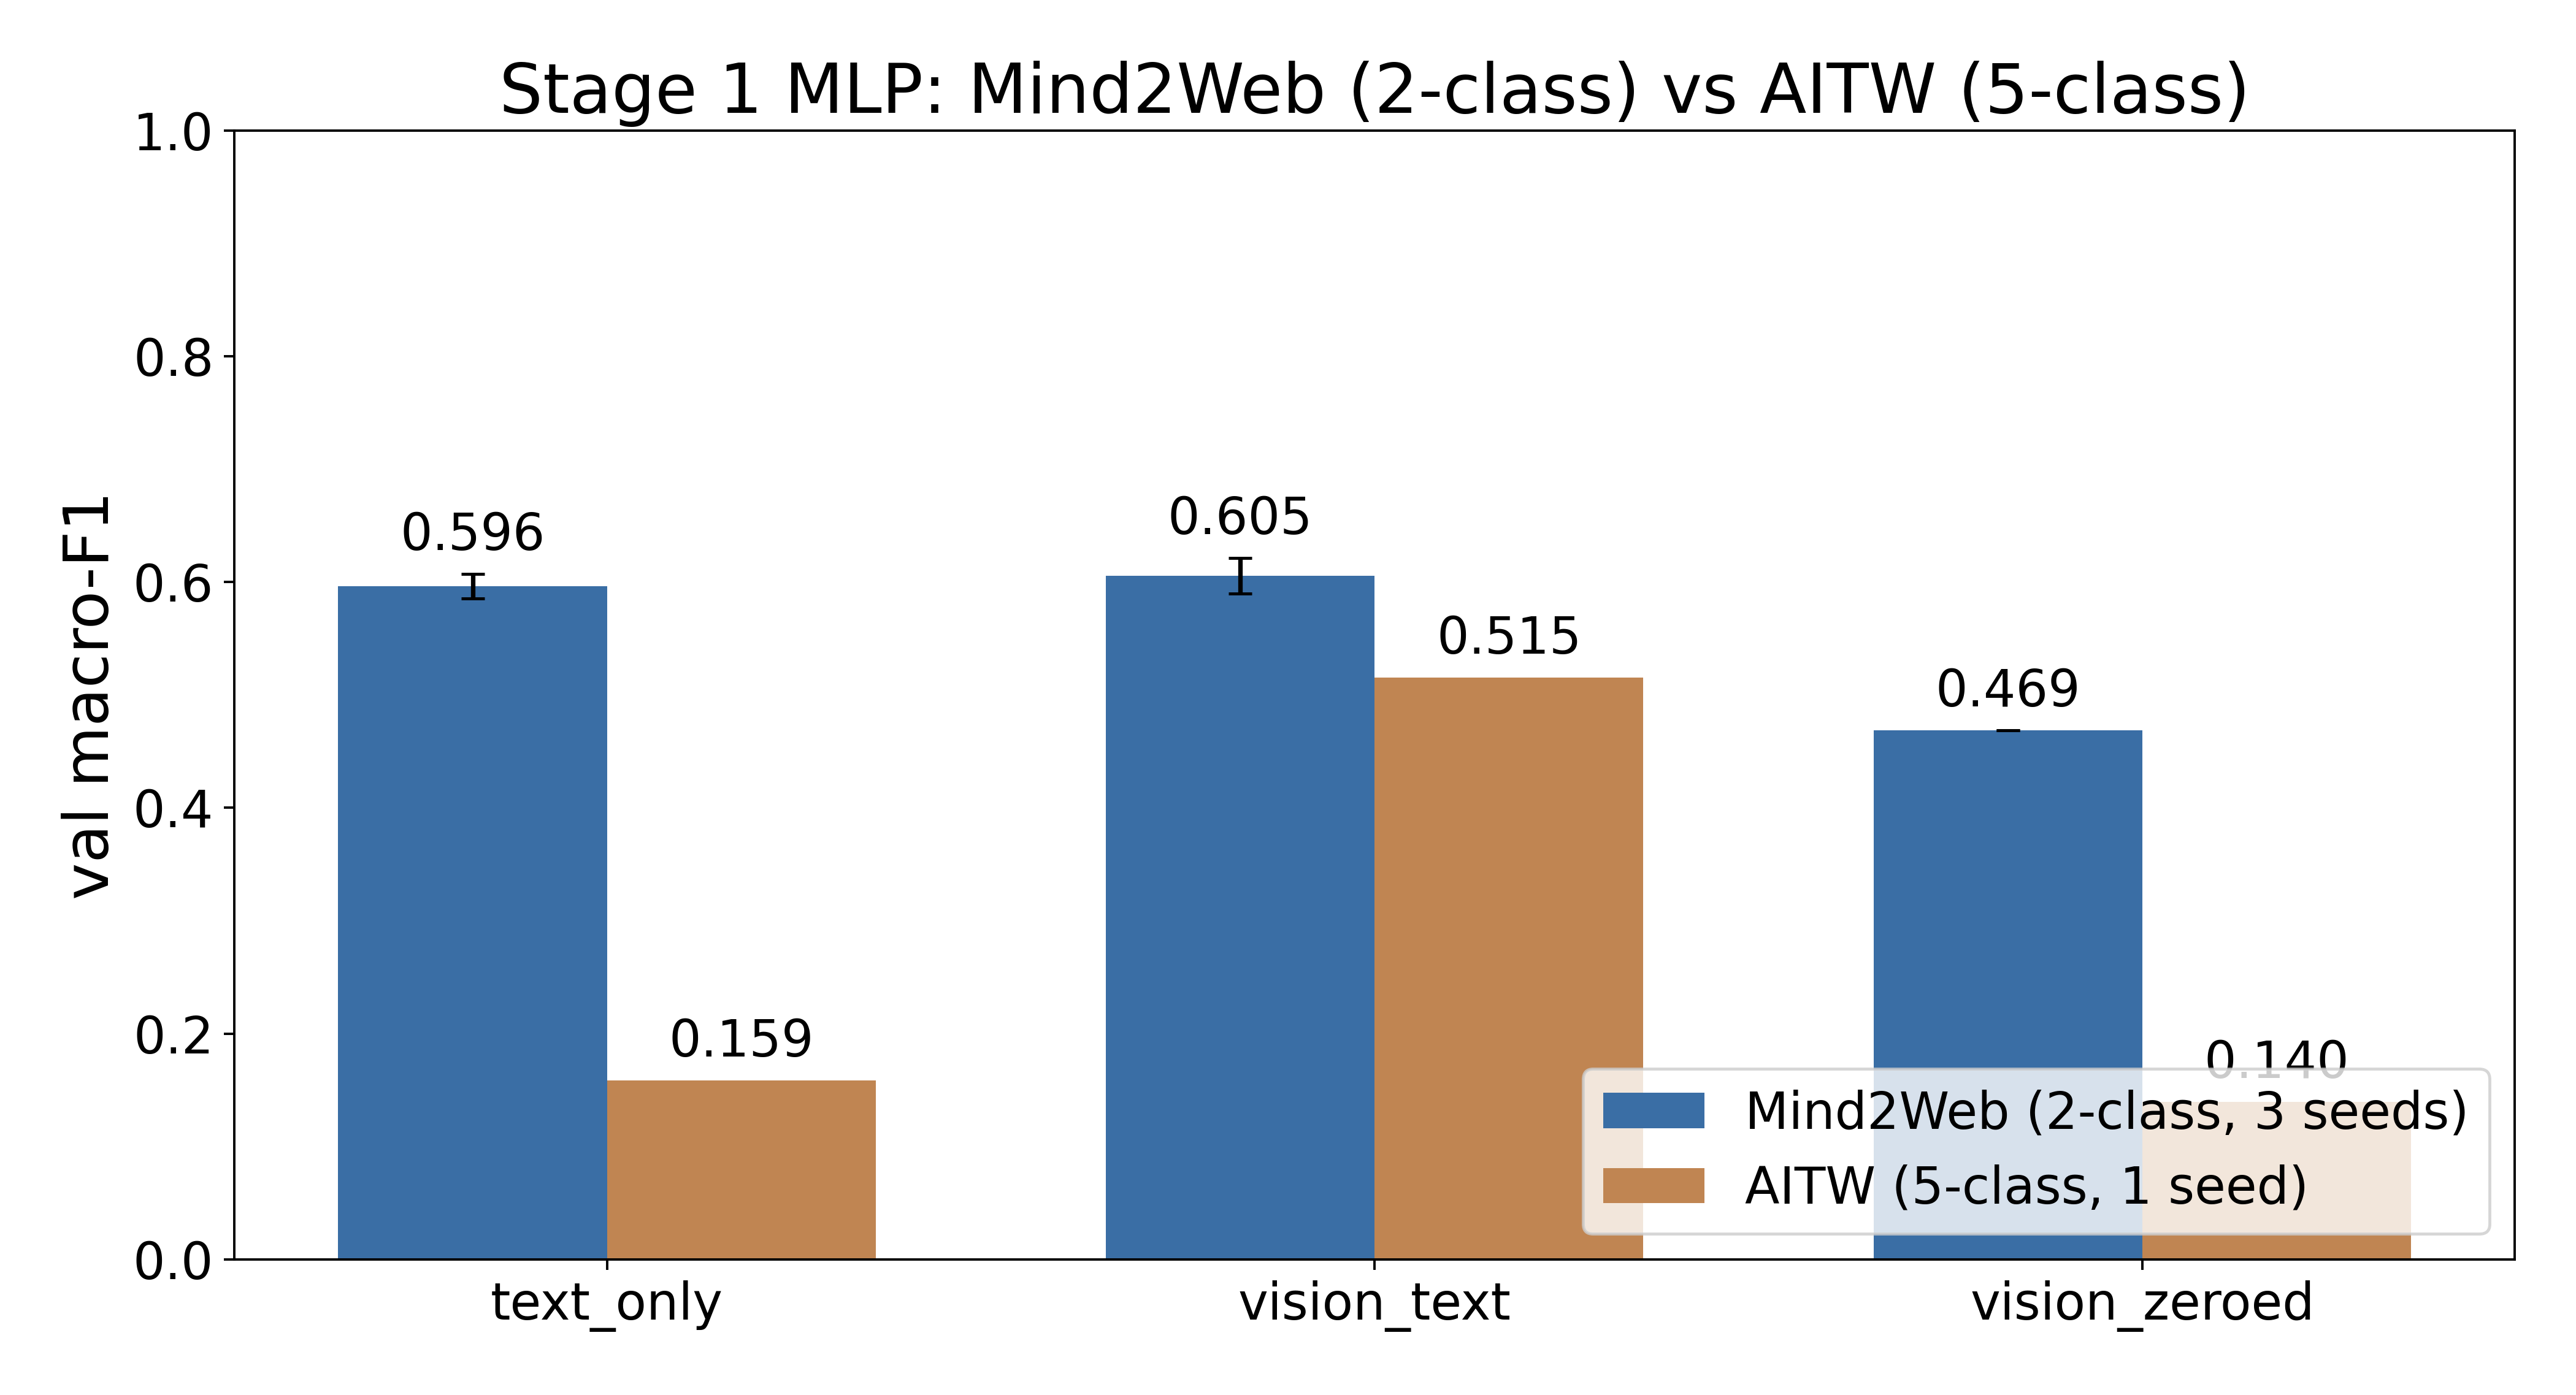
\includegraphics[width=0.98\linewidth]{stage1_mind2web_vs_aitw.png}
\end{center}
\caption{Stage 1 action-type classifier macro-F1 on Mind2Web (2 active
classes) and AITW (5 active classes). Vision is essential on AITW
($+0.414$ over text-only) but redundant on Mind2Web ($+0.009$), because
AITW instructions describe \emph{goals} rather than physically specifying
the action.}
\label{fig:stage1_comparison}
\end{figure}

\section{Related Work}

\textbf{End-to-end GUI agents.} The dominant paradigm treats action type,
arguments, and coordinates as one autoregressive output. UI-TARS~\cite{uitars}
exemplifies this with a unified action space across platforms and explicit
thought traces. OS-Atlas~\cite{osatlas} scales the same paradigm with 13M
cross-platform GUI grounding instances and shows that action-label
harmonization across web/Android/desktop is nontrivial. ShowUI~\cite{showui}
builds a compact VLA around Qwen2-VL with interleaved vision-language-action
streaming. Our flat baseline (Variant~A) replicates the joint-decoding
paradigm of these systems.

\textbf{Modular grounding.} SeeClick~\cite{seeclick} argues that grounding
is the central bottleneck in visual GUI agents. UGround /
SeeAct-V~\cite{uground} separates planning from grounding at the
text-vs-pixel boundary. GUI-Actor~\cite{guiactor} replaces coordinate-token
regression with an attention-based action head driven by a dedicated
\texttt{<ACTOR>} token plus a verifier. Our work studies a different module
boundary: between \emph{action-type prediction} and \emph{spatial
grounding}, not between planning text and coordinates.

\textbf{Reward decomposition.} UI-R1~\cite{uir1} applies RL fine-tuning
with a rule-based reward that separates action-type accuracy from
action-argument accuracy on AndroidControl. It is the closest training
analog: type and location as separable optimization targets; we use
supervised conditioning rather than RL. RegionFocus~\cite{regionfocus}
refines grounding at inference; we change the training-time conditioning
pathway. SayCan~\cite{saycan} and ReAct~\cite{react} provide the
modular-decision precedent, and RT-2~\cite{rt2} the unified token-level
action generation paradigm we critically examine.

\textbf{Evaluation integrity.} Our methodological findings echo, in a GUI
setting, long-standing concerns about test-set contamination and
dependence-blind inference: grouped data require grouped splits and
cluster-aware uncertainty, and repeated measurements of the same example
must not be pooled as independent evidence. Mind2Web's own metric design
(element accuracy vs.\ operation F1 vs.\ step success)~\cite{mind2web}
reflects the type/location decomposition we study.

\section{Data and Splits}

\subsection{Sources and preprocessing}

We use two datasets under a canonical 8-class action taxonomy
(\emph{click}, \emph{double\_click}, \emph{type}, \emph{scroll},
\emph{drag}, \emph{hotkey}, \emph{wait}, \emph{finished}).

\textbf{AITW}~\cite{aitw} (via the \texttt{cjfcsjt/AITW\_General}
HuggingFace mirror, revision pinned to \texttt{5c0dc713}) is the primary
Stage-2 benchmark: five active classes (click 55\%, scroll 13\%, finished
12\%, type 11\%, hotkey 9\%). Screenshots in the mirror are raw RGB bytes
without headers; we decode them against seven observed resolutions with a
portrait-aspect fallback. \texttt{DUAL\_POINT} events are split into taps
(click) versus swipes (scroll) by normalized touch--lift distance
(threshold 0.04). Two data mixes matter below: \texttt{all\_with\_coords}
(tap, swipe, type -- action type is spatially predictive because taps
target small elements while swipes are gestures) and
\texttt{taps\_and\_swipes} (a control where knowing the type carries
little information about \emph{where}).

\textbf{Mind2Web}~\cite{mind2web} (multimodal release) provides the
Stage-1 cross-dataset comparison and a Stage-2 cross-dataset control; it
is click/type-dominated with only two active classes at scale.

\textbf{Coordinates.} Targets are normalized to $[0,1]^2$ and rendered as
the string \texttt{"(x, y)"} on a $[0,999]$ grid; training loss is masked
to the coordinate tokens.

\subsection{Two evaluation protocols}
\label{sec:protocols}

\textbf{Exploratory protocol (Phases 1--7, historical).} Our original runs
streamed the AITW training split in mirror order, filtered by data mix, and
took \emph{consecutive slices}: the first $n_{\text{train}}$ steps for
training and the next $n_{\text{val}}$ for validation. This is the kind of
split that looks innocuous in code review and is not: episodes and,
worse, repeated task goals straddle the boundary
(Section~\ref{sec:leakage}). Every historical number in this paper is
labeled exploratory and is re-analyzed with dependence-aware statistics.

\textbf{Confirmatory protocol (Phase 9, frozen).} We rebuilt the data
pipeline around a frozen manifest: the first 12{,}000
\texttt{all\_with\_coords} steps of the pinned mirror revision, grouped by
\emph{normalized task goal} (episodes never span goals), split
goal-disjointly into train (9{,}511 steps), validation (1{,}660), and an
\textbf{untouched test region} (829): test groups are drawn exclusively
from beyond stream index 5{,}500, past the furthest index any historical
run ever loaded (5{,}250), so no test step was trained on, evaluated on,
or inspected during the exploratory phase. Evaluation sets are frozen and
identical for every variant and training size (250 validation / 600 test
steps for \texttt{all\_with\_coords}; 200/400 for the control mix);
training subsets are nested prefixes. The manifest, split hashes, 17
disclosed near-duplicate goal pairs (token Jaccard $\geq 0.8$), duplicate
checks, and the prespecified analysis (contrasts, metrics, corrections,
failed-run rules) were committed to version control \emph{before} any
test-set evaluation ran. We claim ``decisions frozen before test access,''
documented by commit history -- not third-party preregistration.

\section{Methods}

\subsection{Stage 1: action-type classifier}

A \emph{frozen} Qwen2-VL-2B encodes screenshot+instruction; mean-pooled
final hidden states (1536-d) feed a 3-layer MLP trained with
class-weighted cross-entropy (AdamW, lr $10^{-4}$, batch 128, 8 epochs,
best epoch by validation macro-F1). Modes: \texttt{text\_only} vs.\
\texttt{vision\_text}.

\subsection{Stage 2: five conditioning mechanisms}

Stage~2 fine-tunes Qwen2-VL-2B with LoRA (rank 16 on q/k/v/o projections,
$\approx$0.2\% of parameters) to emit the coordinate string; all variants
share data, optimizer (lr $2\times10^{-5}$, 2 epochs, batch 1), and
evaluation. The only difference is how action-type information enters:

\textbf{A (flat baseline).} No conditioning; replicates joint decoding.

\textbf{B (auxiliary loss).} A linear action-type head on the pooled
representation adds cross-entropy to the grounding loss
($\lambda{=}1$); \emph{no action information at inference}.

\textbf{C (hard routing).} Trained to emit ``\texttt{\{word\} (x, y)}'';
at inference the gold action word is forced as the decode prefix.

\textbf{D-hook (additive embedding).} A learned table
$E\in\mathbb{R}^{8\times d}$; the row for the current action type is added
to \emph{all} token embeddings via a forward hook, preserving the normal
\texttt{input\_ids} path (embedding norm at convergence $\approx0.07$ at
the headline setting).

\textbf{D-token (prepended token -- the original hypothesis).} A sentinel
\texttt{<|action\_slot|>} token is prepended to the instruction and its
embedding replaced in place by $E[a]$, M-RoPE-correctly (the token is in
\texttt{input\_ids}); norm at convergence $\approx2.2$, a strong routable
signal.

\paragraph{Objective.} With screenshot $s$, instruction $g$, action type
$a$, coordinate tokens $y_{1:T}$ and variant-specific conditioning $c$:
\begin{equation}
\mathcal{L}_{\mathrm{coord}} = -\sum_{t=1}^{T} \log
p_\theta\!\big(y_t \mid y_{<t},\, s,\, g,\, c\big),
\label{eq:coord}
\end{equation}
with $c=\varnothing$ for A and B, $c=E[a]$ for D-hook/D-token, and the
forced word for C; B adds $\lambda\,\mathrm{CE}(h_\phi(\bar z), a)$
(Eq.~\ref{eq:coord} otherwise unchanged).

\paragraph{End-to-end pipeline.} The deployable configuration trains
D-hook, then a small MLP head on frozen-backbone features (Stage 1
in-job), and evaluates grounding under \emph{predicted} types; gold-type
results are oracle ceilings, never deployable claims.

\subsection{Evaluation metrics}

\textbf{hit@$r$}: fraction of predictions within normalized L2 distance
$r$ of the target ($r\in\{0.05,0.10,0.25\}$; headline $0.10$).
\textbf{Mean L2}: mean normalized distance (parse failures scored at the
$\sqrt{2}$ sentinel and counted as misses; parse rates reported).
Statistical methodology is Section~\ref{sec:stats}.

\section{Three Evaluation Pitfalls, Quantified}
\label{sec:pitfalls}

\subsection{Pitfall 1: M-RoPE vs.\ \texttt{inputs\_embeds}}
\label{sec:mrope}

Qwen2-VL assigns 3D (temporal, height, width) position IDs to visual
tokens via an \texttt{input\_ids}-keyed path. Our first D-token
implementation injected the action embedding by passing
\texttt{inputs\_embeds} directly, which silently bypasses that path:
image-token positions were computed without the action slot in the
sequence, misaligning multimodal position embeddings for \emph{every}
visual token. The observed effect was a confident $8\sigma$ ``A beats D''
result -- a pure artifact. Rebuilding the same mechanism through the
\texttt{input\_ids} path (D-hook, D-token) erased the deficit. Any
conditioning study on M-RoPE-family models that touches
\texttt{inputs\_embeds} should verify position-ID computation explicitly;
the artifact is silent, large, and directionally misleading.

\subsection{Pitfall 2: stream-slice splits leak task goals}
\label{sec:leakage}

Table~\ref{tab:leakage} quantifies the historical protocol's leakage by
reconstructing, for every historical cell, which episodes and normalized
task goals each validation step shared with that cell's training slice.
Episode-level overlap -- the leakage one usually checks -- is small
(\LeakEpMain{} at the headline cell). The dominant channel is
\emph{shared task goals}: \LeakGoalMain{} of headline validation steps
have a goal string that also appears in training, rising to \LeakGoalMax{}
at $n_{\text{train}}{=}5000$ -- AITW goals repeat across many episodes, so
consecutive-slice splitting almost guarantees template overlap at scale.
Val-set difficulty therefore varies with $n_{\text{train}}$ (each size had
a different val slice), quietly confounding the historical scaling curve.
The confirmatory protocol removes both channels by construction
(goal-disjoint splits; Section~\ref{sec:protocols}).

\begin{table}[tb]
\begin{center}\small
% AUTO-GENERATED by scripts/p10_render_paper_tables.py — do not edit
\begin{tabular}{lccc}
\toprule
historical cell & val steps & sharing a train episode & sharing a train goal \\
\midrule
all\_wc, $n{=}300$ & 250 & 4 (2\%) & 14 (6\%) \\
all\_wc, $n{=}500$ & 250 & 4 (2\%) & 47 (19\%) \\
all\_wc, $n{=}800$ & 250 & 5 (2\%) & 49 (20\%) \\
all\_wc, $n{=}1200$ & 250 & 4 (2\%) & 61 (24\%) \\
all\_wc, $n{=}2500$ & 250 & 10 (4\%) & 133 (53\%) \\
all\_wc, $n{=}5000$ & 250 & 2 (1\%) & 213 (85\%) \\
taps\_swipes, $n{=}1000$ & 200 & 0 (0\%) & 48 (24\%) \\
\bottomrule
\end{tabular}

\end{center}
\caption{Leakage in the historical (exploratory) splits: fraction of
validation steps sharing an episode or a normalized task goal with that
cell's training slice. Goal sharing, not episode straddling, is the
dominant channel.}
\label{tab:leakage}
\end{table}

\subsection{Pitfall 3: pseudo-replicated significance}
\label{sec:stats}

Our original headline significance pooled per-example distances across
seeds -- treating $3\times250$ (seed, example) rows as 750 independent
paired observations. Predictions of the same example by different seeds
are strongly correlated, and examples within an episode share state; the
pooled bootstrap therefore overstates evidence. On synthetic nulls
matching the data's dependence structure (episode and example effects
shared across seeds; zero true difference), the pooled test rejects
\TypeIPooled{} of the time at nominal 5\% (\TypeISims{} simulations),
while the replacement below achieves \TypeIClustered{}.

\textbf{Repaired inference.} For each contrast we (i) average each
example's paired difference over seeds, (ii) cluster examples by episode,
(iii) bootstrap clusters (10{,}000 resamples) for 95\% CIs, and (iv) use
an episode-level sign-flip permutation test (10{,}000 permutations;
$p$-values reported no smaller than Monte Carlo resolution -- never
$p{=}0$). \textbf{Estimand.} This tests the \emph{fixed trained
checkpoints} on new data from the eval population. It is \emph{not}
calibrated for claims about the training procedure: adding run-level
(seed) offsets to the synthetic null drives the episode-clustered test to
\TypeIProc{} rejection (and the pooled test to 70\%). With only three
seeds per variant we therefore
report per-seed means everywhere and make no procedure-level significance
claims. The retracted pooled $p$-values (including a headline
$p{=}\ExpBvsApooled$) should not be cited.

\section{Exploratory Results (historical splits, repaired statistics)}
\label{sec:exploratory}

All numbers in this section come from the leaky historical splits and are
therefore \emph{exploratory}; they are shown with episode-clustered
statistics, and Section~\ref{sec:confirmatory} gives the prespecified
untouched-test versions of every primary claim.

\subsection{Stage 1: vision is essential exactly where instructions
under-specify the action}

\begin{table}[tb]
\begin{center}
\small
\begin{tabular}{lcc}
\toprule
Variant & Mind2Web & AITW \\
 & macro-F1 & macro-F1 \\
\midrule
text\_only & $0.597 \pm 0.011$ & $0.141 \pm 0.032$ \\
vision\_text & $\mathbf{0.605 \pm 0.016}$ & $\mathbf{0.555 \pm 0.036}$ \\
vision\_zeroed & $0.469 \pm 0.000$ & $0.110 \pm 0.051$ \\
\midrule
Vision delta & $+0.009$ & $+0.414$ \\
TF-IDF + LogReg & $0.622$ & $0.168$ \\
Majority floor & $0.472$ & $0.140$ \\
\bottomrule
\end{tabular}
\end{center}
\caption{Stage~1 action-type classification (3 seeds, mean$\pm$std;
exploratory splits). On Mind2Web the instruction text alone contains the
action type; on AITW it does not, and vision contributes $+0.414$
macro-F1. \texttt{vision\_zeroed} collapsing to the majority floor is the
sanity check that features, not priors, drive the result.}
\label{tab:stage1}
\end{table}

Table~\ref{tab:stage1} and Figure~\ref{fig:stage1_comparison}: on
Mind2Web, instructions name the action (``click the submit button''), so
vision adds $+0.009$ macro-F1 over text; on AITW, instructions state goals
(``open a new Chrome private window''), text-only collapses toward the
majority class, and vision adds $+0.414$. A TF-IDF ceiling of $0.168$ on
AITW confirms text is uninformative there regardless of classifier
strength. This asymmetry decides where Stage-2 conditioning could matter
at all.

\subsection{Main ablation under clustered statistics}

\begin{table}[tb]
\begin{center}\small
% AUTO-GENERATED by scripts/p10_render_paper_tables.py — do not edit
\begin{tabular}{lcccc}
\toprule
variant & hit@0.10 & mean L2 $\downarrow$ & $\Delta$ hit@0.10 vs.\ A [95\% CI] & perm.\ $p$ \\
\midrule
A (flat) & $0.255 \pm 0.021$ & $0.392$ & --- & --- \\
B (aux loss) & $0.305 \pm 0.012$ & $0.362$ & $+0.051$ [+0.020, +0.081] & $0.0043$ \\
C (hard routing) & $0.279 \pm 0.032$ & $0.412$ & $+0.024$ [-0.016, +0.063] & $0.278$ \\
D-hook (additive) & $0.300 \pm 0.028$ & $0.365$ & $+0.045$ [+0.011, +0.085] & $0.0227$ \\
D-token (prepended) & $0.269 \pm 0.025$ & $0.375$ & $+0.015$ [-0.018, +0.047] & $0.437$ \\
\bottomrule
\end{tabular}

\end{center}
\caption{Exploratory main ablation (AITW \texttt{all\_with\_coords},
$n_{\text{train}}{=}1200$, 3 seeds, historical leaky splits).
Episode-clustered $\Delta$ vs.\ A with 95\% cluster-bootstrap CIs and
sign-flip permutation $p$. Under the repaired analysis, B survives
(Holm-adjusted $p=\ExpBvsAHolm$ across the four vs.-A contrasts); D-hook
is marginal after correction (Holm $p=\ExpDhvsAHolm$); C and D-token are
not significant.}
\label{tab:exploratory}
\end{table}

Table~\ref{tab:exploratory} re-scores the historical headline with the
repaired statistics (per-seed values in Figure~\ref{fig:ablation}). Three
observations. First, the auxiliary-loss effect
survives: B$-$A on hit@0.10 is \ExpBvsA{} ($p=\ExpBvsAp$), where the
invalid pooled analysis had claimed $p=\ExpBvsApooled$ -- the conclusion
stands but the evidence was overstated by an order of magnitude. Second,
D-hook weakens to marginal after multiplicity correction. Third, the
comparison our proposal cared about most -- D-token vs.\ B -- is
\emph{no longer significant} (\ExpDtvsB{}, $p=\ExpDtvsBp$): on the
historical data we cannot even claim the prepended embedding is
significantly \emph{worse} than the auxiliary loss, only that it shows no
sign of being better.

\begin{figure}[t]
\begin{center}
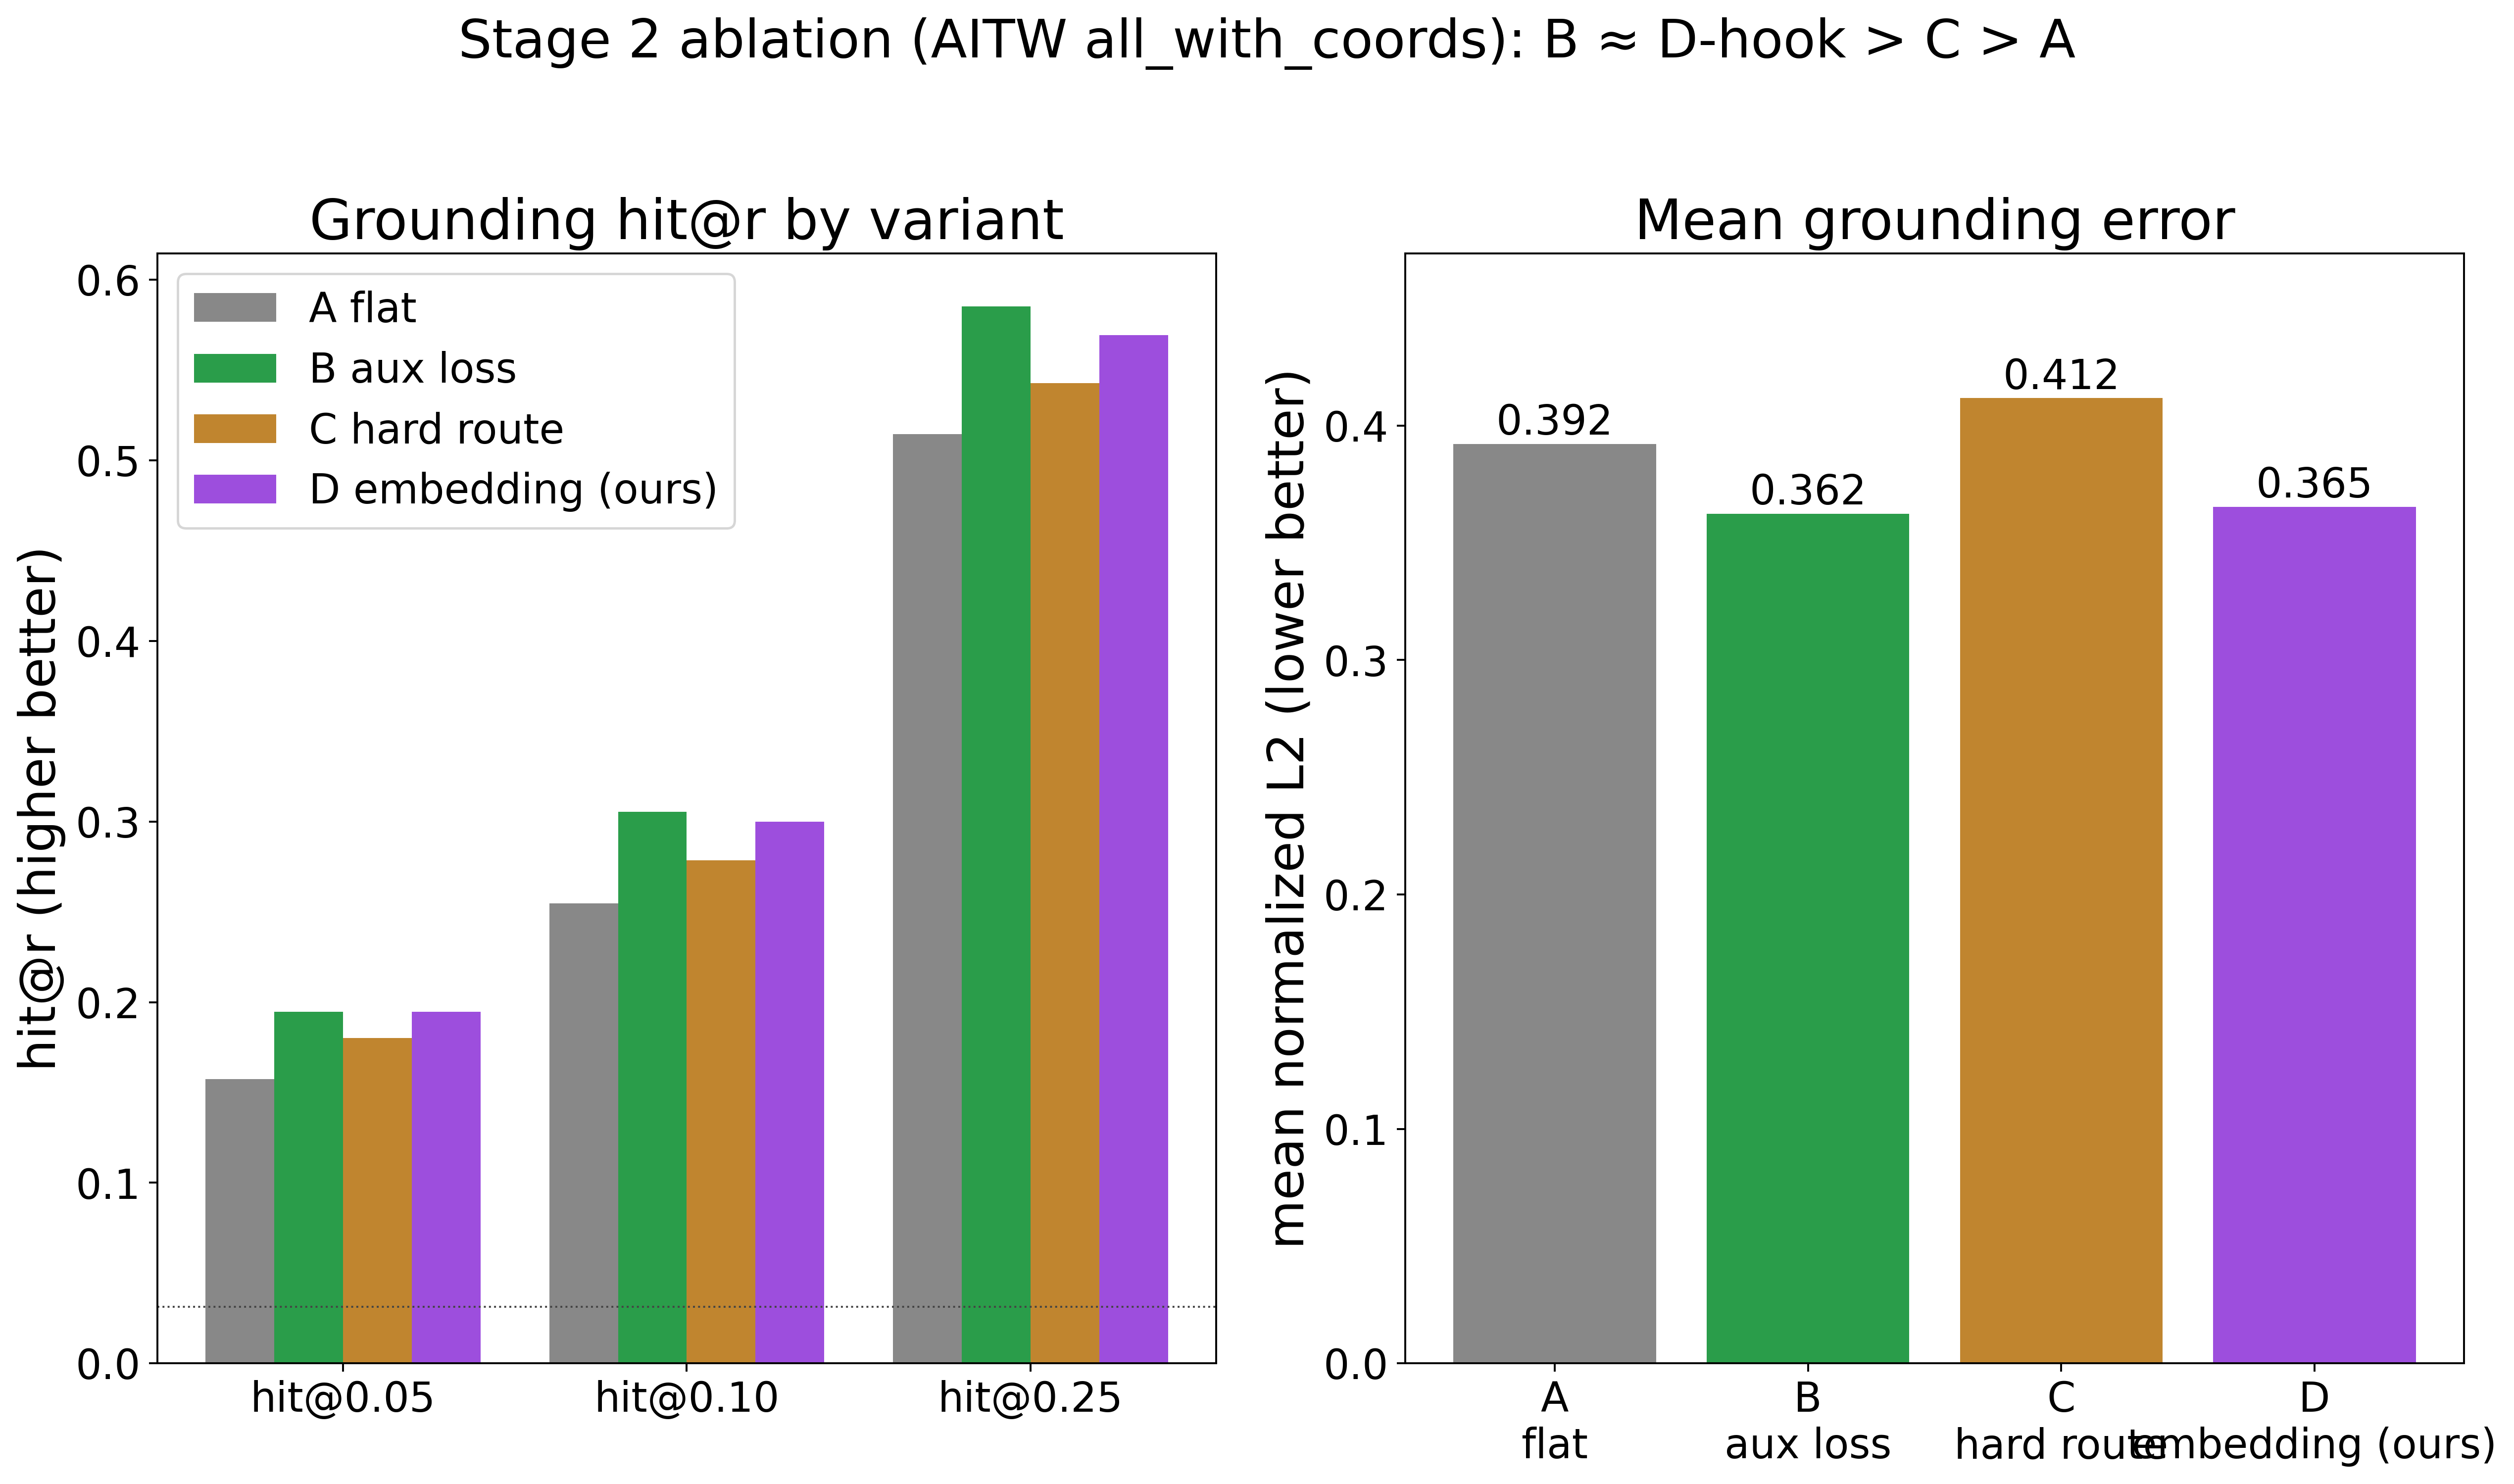
\includegraphics[width=0.98\linewidth]{ablation_ABCD_all_with_coords.png}
\end{center}
\caption{Exploratory ablation on \texttt{all\_with\_coords} (historical
splits; per-seed values). Shown for continuity with the historical record;
Table~\ref{tab:exploratory} carries the calibrated statistics and
Table~\ref{tab:confirmatory} the confirmatory test-set versions.}
\label{fig:ablation}
\end{figure}

\subsection{Per-class decomposition: the gain is click disambiguation}
\label{sec:perclass}

\begin{figure}[t]
\begin{center}
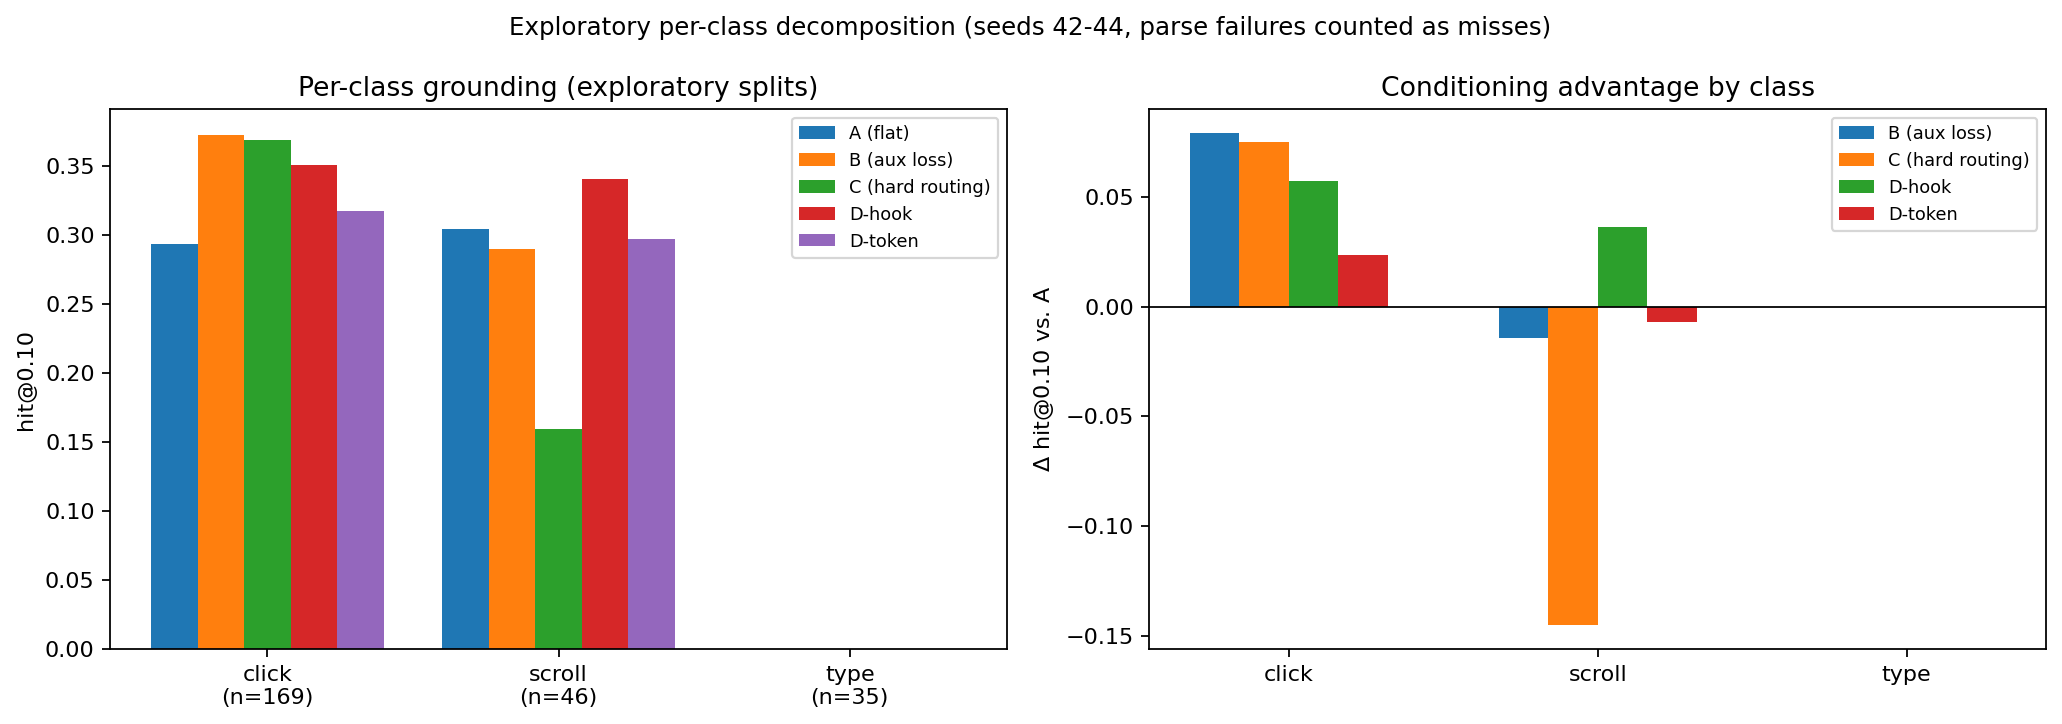
\includegraphics[width=0.98\linewidth]{compounding_error_per_class.png}
\end{center}
\caption{Exploratory hit@0.10 by action class (\texttt{all\_with\_coords}).
The conditioning advantage concentrates in \emph{click}; \emph{type} is
degenerate on AITW (all variants score exactly 0.000, mean L2 at the
$\approx\sqrt{2}$ corner-to-corner distance).}
\label{fig:perclass}
\end{figure}

Breaking hit@0.10 down by class (Figure~\ref{fig:perclass}): B gains
$+0.120$ on click (68\% of examples) with a small scroll cost; C has the
largest click gain ($+0.122$) but destroys scroll ($-0.144$) by forcing a
decode prefix that derails the gesture class; D-hook alone improves both
(click $+0.058$, scroll $+0.039$). The \emph{type} class scores exactly
$0.000$ across all variants with mean normalized L2 at or slightly above
$\sqrt{2}$, the corner-to-corner distance (a few predictions land outside
the unit square): AITW \texttt{type} events carry degenerate touch
coordinates and are ungroundable by any model. This corrects our earlier
``type$\to$text-field localization'' interpretation: the real signal is
\textbf{click-vs-scroll/type disambiguation} for the precise-target class,
and the ``type'' rows merely add a constant drag that cancels in deltas.

\subsection{Control conditions}

On \texttt{taps\_and\_swipes} (action type spatially uninformative), the
historical 3-seed means show no conditioned variant meaningfully above A
(A $0.390{\pm}0.008$, D-hook $0.392{\pm}0.035$ -- a difference well inside
one seed-std -- with B $0.368{\pm}0.009$ and C $0.325{\pm}0.032$ at or
below A on hit@0.10); per-example logs were not retained for A on
this mix, so the clustered version of this control appears only in the
confirmatory rerun (Table~\ref{tab:control}). On Multimodal-Mind2Web
(click/type-dominated), D-hook vs.\ A was $-0.006$ hit@0.10 / $+0.018$
hit@0.25 over 2 seeds -- a null, retained here deliberately: conditioning
does not help where action type carries no spatial information, on either
dataset.

\subsection{Low-data behavior: no clean curve}
\label{sec:lowdata}

\begin{figure}[t]
\begin{center}
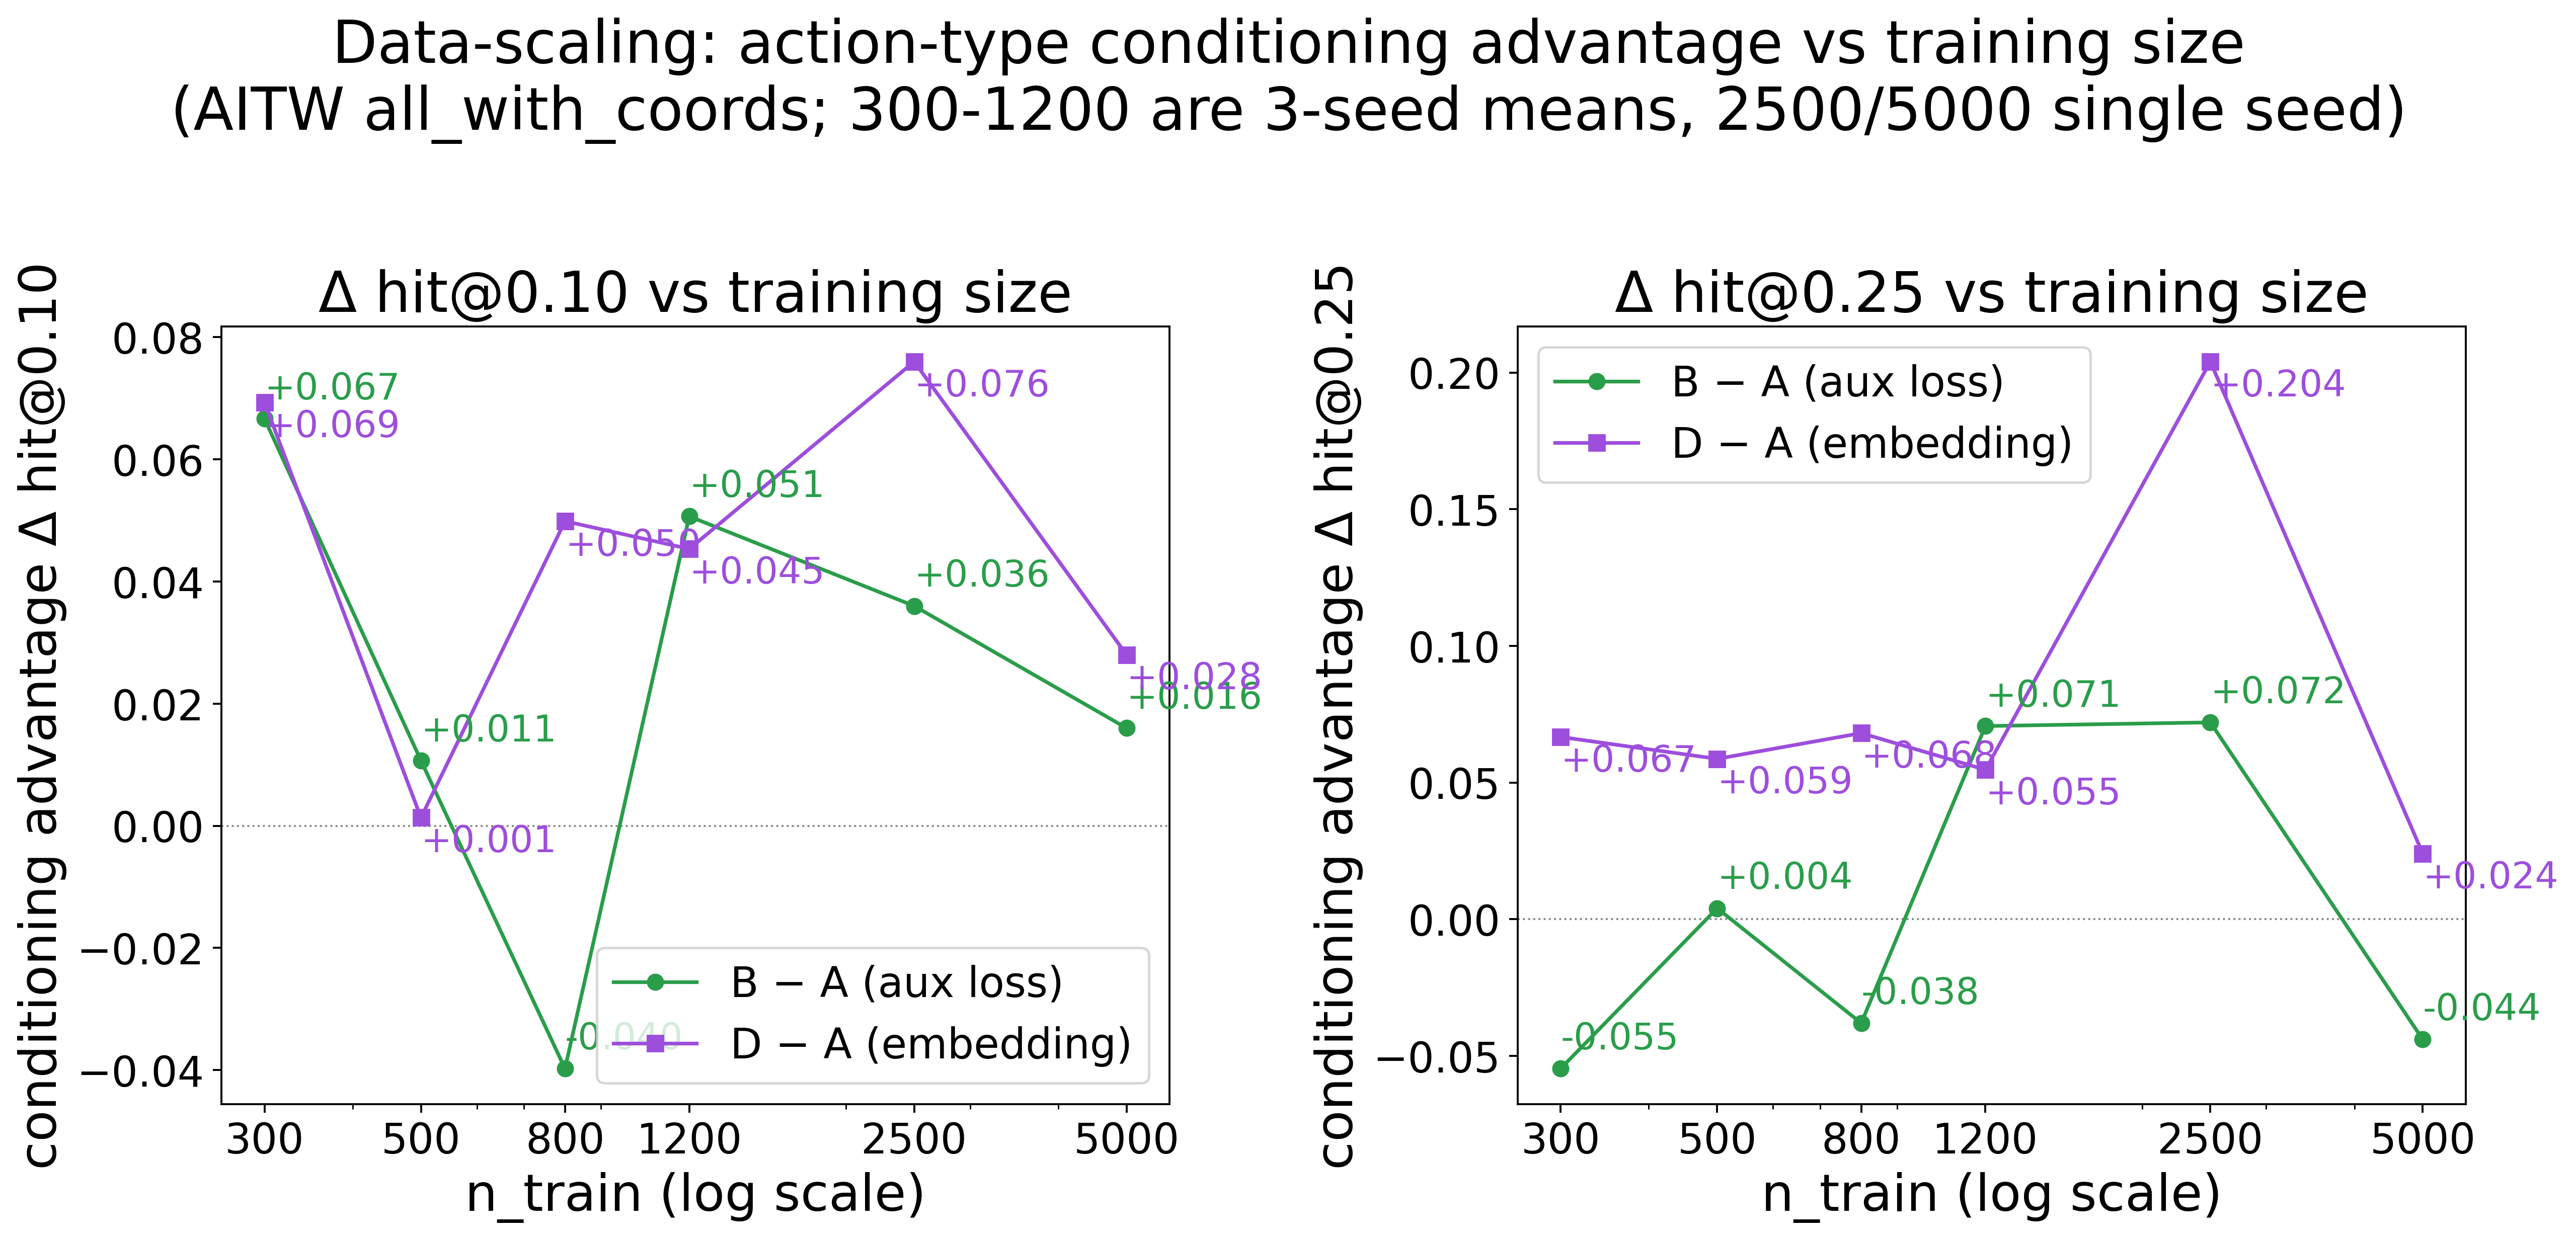
\includegraphics[width=0.98\linewidth]{scaling_curve.png}
\end{center}
\caption{Exploratory conditioning advantage ($\Delta$ hit@0.10 vs.\ A)
across $n_{\text{train}}$. Caveat from Section~\ref{sec:leakage}: each
historical size used a \emph{different} val slice with different goal
leakage (up to \LeakGoalMax), so this curve is directional at best; the
confirmatory grid (Table~\ref{tab:lowdata}) fixes one frozen test set for
all sizes.}
\label{fig:scaling}
\end{figure}

Our proposal predicted the advantage is a low-data prior. The historical
grid ($n\in\{300,500,800\}$, 3 seeds) does \emph{not} show a clean
monotone: B$-$A on hit@0.10 is $+0.067$ at $n{=}300$ but $+0.011$ at
$n{=}500$ and $-0.040$ at $n{=}800$; D-hook is more stable ($+0.069$,
$+0.001$, $+0.048$) and leads hit@0.25 and mean L2 at every low-data size.
The two single-seed high-end cells disagree with each other: at
$n{=}5000$ the deltas shrink and partially reverse (B$-$A hit@0.25 goes
negative), while at $n{=}2500$ D-hook posts the \emph{largest}
conditioning deltas anywhere in the study ($+0.076$ hit@0.10, $+0.204$
hit@0.25) -- single-seed noise on a differently-leaky val slice, cutting
in the direction \emph{favorable} to conditioning. We report all of this
as: \emph{inconclusive on the low-data-prior hypothesis -- noisy,
non-monotone, and confounded by per-size val sets}
(Figure~\ref{fig:scaling}); the prespecified low-data claim is evaluated
on the frozen test set in Section~\ref{sec:confirmatory}. An earlier draft
of this work called the low-data prediction ``confirmed''; that claim did
not survive this audit.

\subsection{The e2e pipeline claim also weakens}

The historical end-to-end result (predicted-type pipeline $0.271$ vs.\ A
$0.255$ hit@0.10) was previously reported as a win. Under clustered
statistics the paired difference is \ExpEtoEPredvsA{}
($p=\ExpEtoEPredvsAp$) -- not significant; the oracle-type version is
marginal (\ExpEtoEOraclevsA). The deployable-pipeline question is
therefore decided by the confirmatory run (P4, below), not the historical
data.

\subsection{D-token causal-use sensitivity}

\begin{table}[tb]
\begin{center}\small
% AUTO-GENERATED by scripts/p10_render_paper_tables.py — do not edit
\begin{tabular}{lccc}
\toprule
contrast & $\Delta$ hit@0.10 [95\% CI] & $\Delta$ hit@0.25 [95\% CI] & perm.\ $p$ (hit@0.10) \\
\midrule
wrong $-$ gold & $-0.192$ [-0.233, -0.149] & $-0.329$ [-0.372, -0.284] & $\leq 9.999e-05$ \\
zero $-$ gold & $-0.093$ [-0.128, -0.059] & $-0.112$ [-0.145, -0.079] & $\leq 9.999e-05$ \\
\bottomrule
\end{tabular}

\end{center}
\caption{Exploratory D-token sensitivity (episode-clustered, 3 seeds):
evaluating the same trained model with wrong or zeroed action embeddings
severely degrades grounding. This establishes the embedding is
\emph{used} at inference -- a sensitivity/oracle analysis, not evidence
that conditioning caused any gain over A.}
\label{tab:causal}
\end{table}

Feeding the trained D-token model a \emph{wrong} action id collapses
grounding, and zeroing the embedding hurts substantially
(Table~\ref{tab:causal}). The refutation of the proposal's mechanism is
therefore precise: the prepended embedding is causally used, it is simply
not the best way to exploit action-type supervision. Figure~\ref{fig:attention}
shows one example where correct conditioning concentrates more attention
mass on the screenshot; across the three examples we probed the pattern is
not uniform, so we present it strictly as illustration, not evidence.

\begin{figure}[tb]
\begin{center}
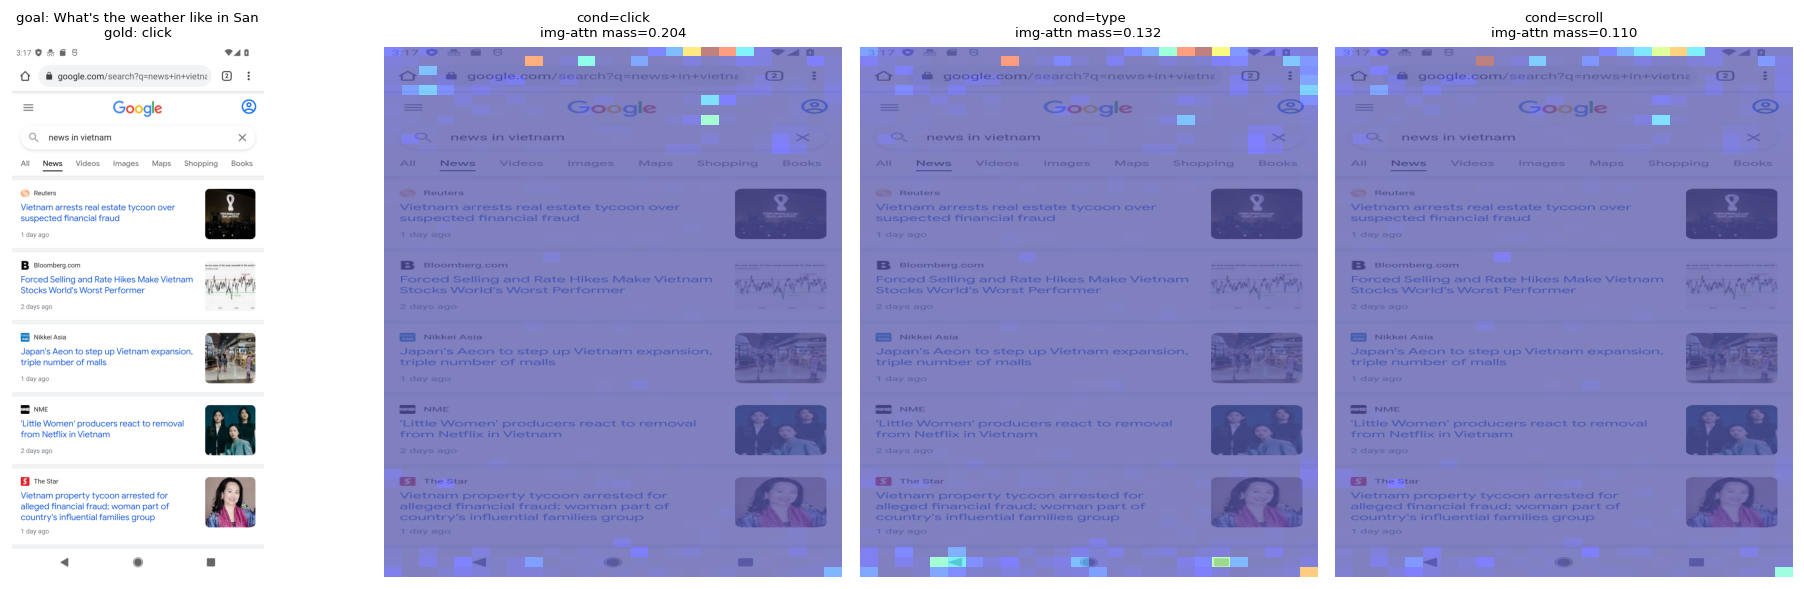
\includegraphics[width=0.98\linewidth]{attn_example_1.png}
\end{center}
\caption{Image-region attention for a held-out \emph{click} example under
three action-type conditionings (qualitative illustration; screenshot
attention mass 0.204 under \emph{click} vs.\ 0.132/0.110 under
\emph{type}/\emph{scroll}).}
\label{fig:attention}
\end{figure}

\section{Confirmatory Results (untouched test, prespecified)}
\label{sec:confirmatory}

All variants were retrained from scratch on the frozen goal-disjoint
splits (identical hyperparameters, seeds 42--44) and evaluated once on the
untouched 600-step test set; the four primary contrasts, the headline
metric (hit@0.10), the clustered test, and Holm correction were committed
before any test evaluation ran (Section~\ref{sec:protocols}).

\begin{table}[tb]
\begin{center}\small
% AUTO-GENERATED by scripts/p10_render_paper_tables.py — do not edit
\begin{tabular}{lcccc}
\toprule
variant & hit@0.10 & mean L2 $\downarrow$ & $\Delta$ hit@0.10 vs.\ A [95\% CI] & perm.\ $p$ (Holm) \\
\midrule
A (flat) & $0.219 \pm 0.018$ & $0.450$ & --- & --- \\
B (aux loss) & $0.230 \pm 0.004$ & $0.445$ & $+0.011$ [-0.005, +0.029] & $0.23$ (0.309) \\
C (hard routing) & $0.219 \pm 0.019$ & $0.498$ & $+0.000$ [-0.022, +0.021] & $1$ \\
D-hook (additive) & $0.276 \pm 0.003$ & $0.376$ & $+0.057$ [+0.035, +0.079] & $<10^{-4}$ (0.0004) \\
D-token (prepended) & $0.265 \pm 0.004$ & $0.388$ & $+0.046$ [+0.027, +0.067] & $0.0002$ \\
\bottomrule
\end{tabular}

\end{center}
\caption{\textbf{Confirmatory} main ablation on the untouched,
goal-disjoint AITW test set ($n{=}600$ steps;
$n_{\text{train}}{=}1200$; 3 seeds; mean$\pm$std across seeds).
$\Delta$ vs.\ A: episode-clustered 95\% CI and permutation $p$
(Holm-adjusted across the four primary contrasts where applicable).}
\label{tab:confirmatory}
\end{table}

\begin{table}[tb]
\begin{center}\small
% AUTO-GENERATED by scripts/p10_render_paper_tables.py — do not edit
\begin{tabular}{lccccc}
\toprule
variant & hit@0.10 & L2 $\downarrow$ & parse & $\Delta$ vs.\ A [95\% CI] & $p$ \\
\midrule
A (flat) & $0.302 \pm 0.009$ & $0.268$ & $100.0\%$ & --- & --- \\
B (aux loss) & $0.316 \pm 0.018$ & $0.264$ & $100.0\%$ & $+0.013$ [-0.013, +0.041] & $0.364$ \\
C (hard routing) & $0.236 \pm 0.064$ & $0.454$ & $84.7\%$ & $-0.067$ [-0.100, -0.039] & $<10^{-4}$ \\
D-hook (additive) & $0.349 \pm 0.020$ & $0.213$ & $100.0\%$ & $+0.047$ [+0.010, +0.079] & $0.0327$ \\
\bottomrule
\end{tabular}

\end{center}
\caption{Confirmatory control mix (\texttt{taps\_and\_swipes}) on its
frozen 400-step test set: when action type is not spatially predictive,
conditioning should not help; this is the falsifiable half of the thesis.}
\label{tab:control}
\end{table}

\begin{table}[tb]
\begin{center}\small
% AUTO-GENERATED by scripts/p10_render_paper_tables.py — do not edit
\begin{tabular}{lccc}
\toprule
$n_{\text{train}}$ & A & $\Delta$ B$-$A [95\% CI] & $\Delta$ D-hook$-$A [95\% CI] \\
\midrule
$n{=}300$ & $0.138$ & $+0.038$ [+0.013, +0.064] & $+0.049$ [+0.025, +0.073] \\
$n{=}500$ & $0.219$ & $-0.004$ [-0.027, +0.018] & $+0.016$ [-0.008, +0.039] \\
$n{=}800$ & $0.256$ & $+0.003$ [-0.014, +0.020] & $+0.036$ [+0.015, +0.057] \\
\bottomrule
\end{tabular}

\end{center}
\caption{Confirmatory low-data grid on the \emph{same} frozen test set for
every training size (nested training prefixes), removing the
per-size-val-set confound of Figure~\ref{fig:scaling}.}
\label{tab:lowdata}
\end{table}

\textbf{P1 (auxiliary supervision).} B vs.\ A on hit@0.10: \ConfBvsA{},
permutation $p=\ConfBvsAp$, Holm $p=\ConfBvsAHolm$; mean-L2 delta
\ConfBvsALtwo{} ($p=\ConfBvsALtwop$).

\textbf{P2 (inference-time conditioning).} D-hook vs.\ A: \ConfDhvsA{}
(Holm $p=\ConfDhvsAHolm$).

\textbf{P3 (the proposal's mechanism).} D-token vs.\ B: \ConfDtvsB{}
(Holm $p=\ConfDtvsBHolm$).

\textbf{P4 (deployable pipeline).} End-to-end predicted-type pipeline
vs.\ A: \ConfEtoEvsA{} (Holm $p=\ConfEtoEvsAHolm$); Stage-1 test accuracy
\ConfStageOneAcc{}, oracle ceiling \ConfEtoEOracle{} vs.\ predicted
\ConfEtoEPred{} (paired gap \ConfEtoEGap).

Secondary contrasts, per-class decompositions, parse rates, and per-seed
values for every run are in the released
\texttt{results/phase9\_rerun/rerun\_analysis.json}; per-seed means for
each primary contrast appear alongside the released analysis, and no
procedure-level significance claim is made from three seeds
(Section~\ref{sec:stats}).

\section{Limitations}

Offline step-level hit@radius is not long-horizon task success: it scores
logged single steps, without interaction, recovery, or compounding-error
dynamics -- the motivating failure mode is measured here only via its
step-level signature. The backbone is a single 2B model; conclusions are
about this scale and training recipe, not about GUI agents generally, and
our baselines are small matched-compute models trained by us, not
state-of-the-art systems.
The confirmatory estimand is fixed checkpoints, not the training
procedure (three seeds; per-seed effects reported). AITW's \texttt{type}
coordinates are degenerate, so ``grounding'' on
\texttt{all\_with\_coords} is effectively click/scroll grounding plus a
constant; the click-concentration analysis is post-hoc on exploratory
data and only its prespecified aggregate versions are confirmatory. Goal
strings are our dependence proxy; 17 near-duplicate train/test goal pairs
(disclosed in the manifest) survive normalization, and subtler sharing
(same app, similar screens) is not modeled. The Mind2Web control used 2
seeds without per-example logs. Finally, the mirror we pin is a
third-party repackaging of AITW; we verified revision stability but not
byte-level provenance against the original release.

\section{Conclusion}

The broad factorization thesis survives careful evaluation in narrowed
form: auxiliary action-type supervision helps a small GUI grounding model
where action type is spatially predictive, the effect concentrates in
click disambiguation, and it disappears on matched controls -- with the
confirmatory test-set verdicts for all four prespecified contrasts
reported above exactly as they came out. The specific architecture our
proposal advocated -- a learned prepended action embedding -- is refuted
as the winning mechanism despite being demonstrably used by the model. En
route we hit, diagnosed, and repaired three evaluation artifacts (a
silent M-RoPE position bug producing an $8\sigma$ false negative;
goal-level split leakage reaching \LeakGoalMax{}; pseudo-replicated
statistics with \TypeIPooled{} measured type-I error), each individually
capable of flipping the paper's conclusion. We suspect none of them is
unique to us: stream-sliced splits, embedding-injection shortcuts, and
pooled per-seed bootstraps are all common patterns. The frozen splits,
per-example predictions, clustered-inference code, and prespecification
are released so both the object-level result and the audit are
reproducible.

%%%%%%%%% CONTRIBUTIONS + GENAI (not counted toward the page limit)
\section*{Contributions}
\textbf{A.~Chauhan}: training and evaluation infrastructure, Stage-2
conditioning variants, cloud experiment orchestration, statistical
reanalysis and confirmatory protocol, writing. \textbf{A.~Ilyasov}:
Stage-1 classifier study, data pipeline and error analysis, figures,
editing. Both authors contributed to problem formulation and experimental
design and approved the final manuscript.

\section*{Generative AI Usage Statement}
Large-language-model assistants (Anthropic Claude) were used extensively
under the authors' direction: writing and debugging training, evaluation,
and statistical-analysis code; orchestrating cloud experiments; drafting
the integrity audit that led to Sections~\ref{sec:pitfalls}
and~\ref{sec:confirmatory}; and drafting and editing this manuscript. The
authors specified the research questions and methodology, reviewed the
analyses, verified reported numbers against the committed result
artifacts (every table is generated programmatically from those
artifacts), and take full responsibility for all content.


\bibliographystyle{ieee}
\bibliography{paper}

\appendix
\section{Method details}
\label{app:methods}
\datasources
\methstageone
\methobjective

\section{Exploratory material (historical splits)}
\label{app:exploratory}
This appendix holds supporting exploratory material referenced from the
main text: the Stage~1 action-type classifier study, the D-token
causal-use sensitivity analysis, and three figures from the historical
(leaky-split) phase. All of it is exploratory and superseded for
inferential purposes by the confirmatory results in the main text.

\tabexploratoryfloat
\tabcontrolfloat
\tablowdatafloat
\expstageone
\expperclass
\explowdata
\expetoe
\expcausal
\figexpablation
\figexpscaling
\figexpattention

\end{document}
